\subsection{Eingesetzte Technologien} \label{sec:technologies}
In dieser Anwendung wird eine App für das mobile \ac{OS} Android implementiert, allerdings wird nicht mit androidspezifischen Werkzeugen entwickelt, sondern mit Webtechnologien. Das Ergebnis kann später einfach auf die gewünschte Zielplattform portiert werden. In diesem Kapitel werden die wichtigsten Technologien kurz vorgestellt. Die Beschreibung ist nicht vollständig, sondern soll lediglich die Kernaspekte der Technologien wiedergeben. Zudem wird kurz erklärt, wofür welche Technologie eingesetzt wird und warum diese genutzt wird. Abbildung \ref{fig:technology_stack} zeigt das Zusammenspiel der Technologien und einen beispielhaften Ablauf der Kommunikation in der Applikation.

\begin{figure}[h]
	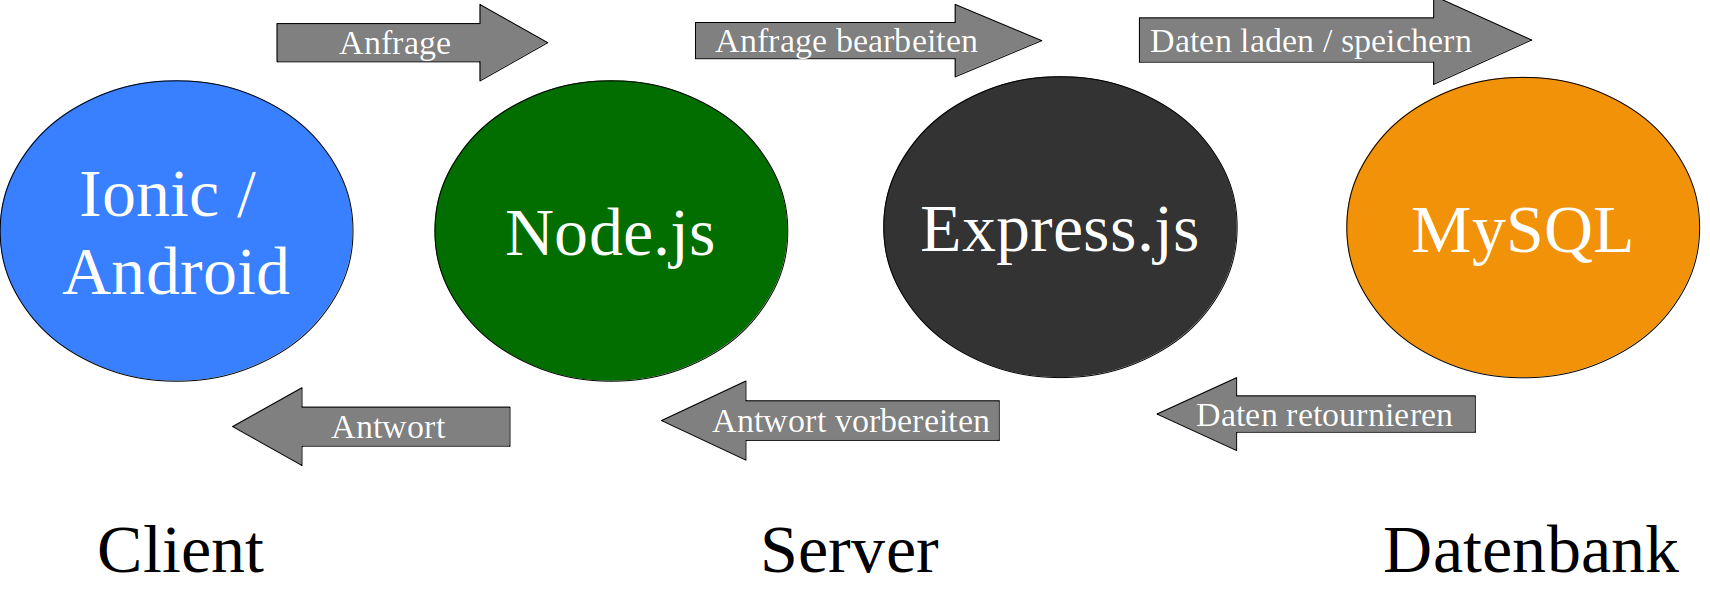
\includegraphics[width=1\linewidth]{figures/development/technologies/technologien}
	\caption{Technologiestack}
	\label{fig:technology_stack}
\end{figure}

\subsubsection{JavaScript (JS)} \label{tec:javascript}
\ac{JS} ist eine clientseitige Skriptsprache, die verwendet wird, um dynamische Webseiteninhalte zu erstellen und zu verwalten. \ac{JS} ist schwach typisiert und verfügt über objektorientierte, sowie funktionale Programmierparadigmen. Mittels \ac{DOM} und \ac{JS} kann jedes \acs{HTML}-Element einfach manipuliert werden. Zudem können Events auf Elementen definiert werden, die durch den/die User/in beliebig ausgelöst werden können (z.B. Klicken auf eine Schaltfläche). \cite{morris:javascript:2019} \\
\ac{JS} wurde als primäre Programmiersprache gewählt, da die Technologie mittlerweile beliebter auf \href{https://github.com/}{Github} und \href{https://stackoverflow.com/}{StackOverflow} ist als Java, Python oder PHP, wie in Abbildung \ref{fig:github_ranking_programming_language} gezeigt wird. Damit ist sichergestellt, dass die Sprache genug Unterstützung aus der Community erhält und Fragen schnell und kompetent in Foren beantwortet werden.

\begin{figure}[h]
	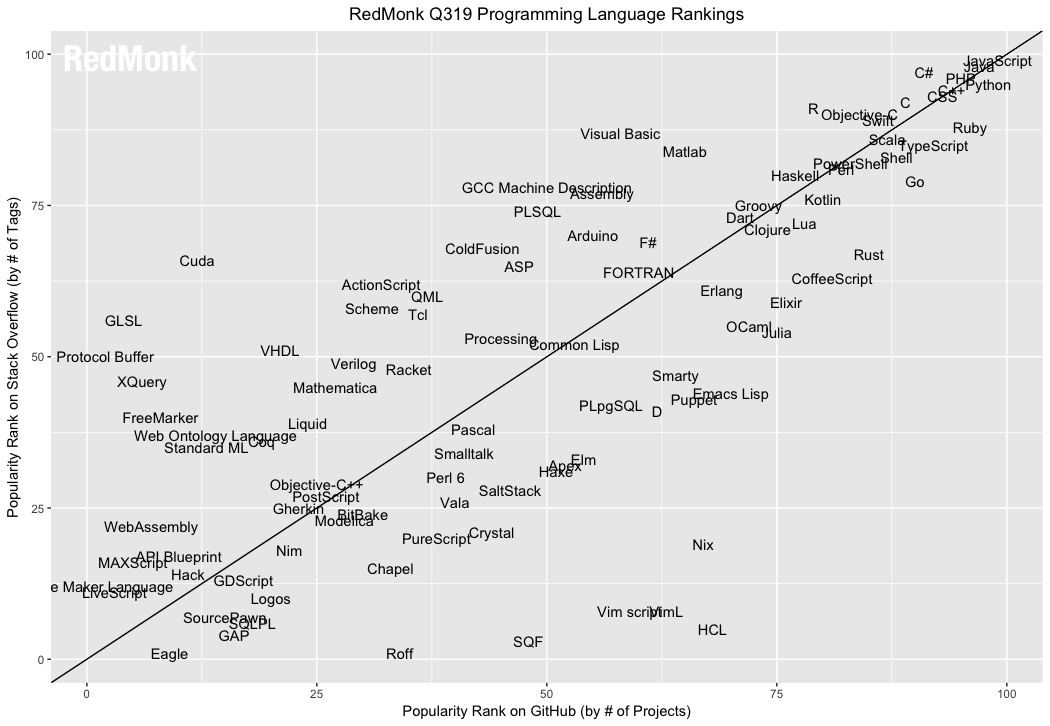
\includegraphics[width=1\linewidth]{figures/development/technologies/programming_language_rank}
	\caption{Popularität der bekannte Programmiersprachen \cite{grady:language_popularity:2019}}
	\label{fig:github_ranking_programming_language}
\end{figure}

\paragraph{Typescript (TS)} \label{tec:typescript}
\ac{TS} ist eine Programmiersprache, die von Microsoft im Jahre 2012 veröffentlicht wurde. \ac{TS} bildet eine Obermenge von \ac{JS}, wodurch \ac{TS} alle Funktionen von \ac{JS} besitzt und noch viele weitere, die in der aktuellen Version noch nicht unterstützt werden. Der größte Vorteil von \ac{TS} ist die statische Typsicherheit, wodurch Variablen ein Datentyp zugewiesen werden kann. Beim Kompilieren werden die zugewiesenen Typen überprüft und Fehler ausgegeben, falls eine falsche Zuweisung entdeckt wurde. Somit können bereits viele Bugs ausgeschlossen werden, bevor die Applikation ausgeführt wurde. Außerdem werden von \ac{TS} objektorientierte Programmierparadigmen unterstützt, welche die Entwicklung von größeren Anwendungen erleichtern sollen. \cite{lease:typescript:2019} \\
\ac{TS} wird aufgrund der insgesamt besseren Wartbarkeit und Verständlichkeit des entwickelten Programmcodes in allen Bereichen der Applikation statt \acl{JS} eingesetzt.

\subsubsection{Node.js} \label{tec:nodejs}
Mithilfe von Node.js kann \ac{JS} serverseitig verwendet werden. Bidirektionale Kommunikation von Client und Server wird von Node.js in Form von Websockets unterstützt. Traditionelle Web-Applikationen erlauben nicht, dass der Server mit dem Client interagiert, falls sich Daten im Hintergrund ändern. Hinzukommend erfolgt die Abarbeitung von I/O Operationen asynchron, damit die Programmausführung nicht unnötig lange blockiert wird. \cite{nodejs:2013}

\paragraph{Express.js} \label{tec:expressjs}
Express.js ist ein Framework, welches auf Node.js aufsetzt und viele integrierte Features und Funktionen für die Entwicklung einer flexiblen \ac{API} bereitstellt. Ein Kernaspekt von Express ist die Performance. \cite{express:2019} \\ 
Express wird als Backend eingesetzt, welches die Webanfragen der App bearbeitet und die spielrelevanten Daten formatiert in die Datenbank ablegt. Express wurde aus dem Grund gewählt, damit beide Teile der Applikation (Front- \& Backend) in einer Programmiersprache entwickelt werden, was die Komplexität deutlich verringert, da einzelne Aspekte ohne zusätzlichen Aufwand wiederverwendet werden können.

\subsubsection{Angular} \label{tec:angular}
Angular ist ein Framework für \ac{JS}, mithilfe dessen \ac{SPAs} einfach entwickelt werden können. \ac{SPAs} aktualisieren sich dynamisch, während der/die Benutzer/in mit ihnen interagiert. Dadurch bieten sie eine bessere Erfahrung, da keine langen Wartezeiten durch das Neuladen der Webseite entstehen. Zudem kann der Code in mehrere wiederverwendbare Module unterteilt werden. Die Testbarkeit ist ein zentraler Punkt des Frameworks. Unterstützt werden Unit- und End-to-End Tests. \cite{goel:angular:2019}\cite{krukowski:angular:2019} 

\paragraph{Ionic} \label{tec:ionic}
Ionic ist ein Toolkit, mit dem hochqualitative Apps und Desktopapplikationen anhand von gängigen Webtechnologien (\ac{HTML}, \ac{CSS} und \ac{JS}) entwickelt werden können. Ionic bietet offizielle Unterstützung für \nameref{tec:angular}, allerdings befindet sich der Support für andere \acl{JS}-Frameworks wie Vue oder React in Entwicklung. Ein Ziel des Frameworks ist es, dass der Source Code nur einmal geschrieben werden muss und dann auf allen möglichen Plattformen (iOS, Android, Windows, Linux, \dots) ausgeführt werden kann. Mithilfe von Ionic können auch plattformspezifische Funktionen der verschiedenen \acl{OS}e angesteuert werden, wie das Neigen des Smartphones. \cite{ionic:2019} \\
Der Grund für den Einsatz von Ionic ist, dass das Framework Wert auf Einfachheit legt, weshalb das Erlernen der Kernfunktionalität sehr simpel ist. Hinzu kommt, dass das Framework mit einer Menge vorgefertigter Komponenten ausgeliefert wird, die ohne weitere Konfiguration verwendbar sind, wodurch eine Weboberfläche zusammengestellt werden kann. 

\subsubsection{Android} \label{tec:android}
Android ist ein Linux-basiertes \ac{OS}, welches von Google entwickelt und betreut wird. Hauptsächlich kommt Android auf Smartphones zum Einsatz, jedoch gibt es auch angepasste Versionen für Uhren und Fernseher. Die Software ist mit rund 76\% Verbreitung im Juli 2019 das beliebteste mobile \ac{OS} der Welt.
\cite{android:2019}\cite{android:marketshare:2019} \\
Aufgrund der sehr großen Verbreitung und der Beliebtheit wurde Android als primäres Betriebssystem für die App gewählt. Diese Umstände bieten noch weitere Vorteile, denn das Projekt wird aufgrund der Popularität vermutlich noch lange weitergeführt. Zudem wendet Google immense Ressourcen für die Weiterentwicklung und Verbesserung des Systems auf.

%\begin{figure}[h]
%	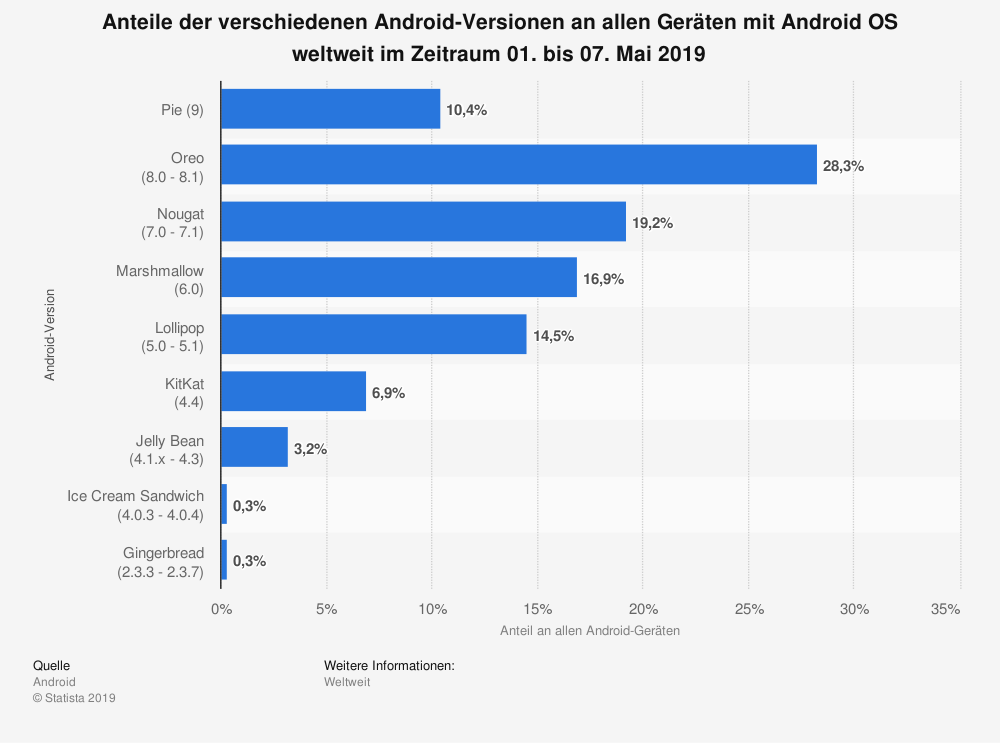
\includegraphics[width=1\linewidth]{figures/development/technologies/android_versionverbreitung}
%	\caption{Anteile der verschiedenen Android-Versionen an allen Geräten mit Android OS weltweit im Zeitraum 01. bis 07. Mai 2019 \cite{android:distribution:2019}}
%	\label{fig:android_distribtuon}
%\end{figure}

\subsubsection{MySQL} \label{tec:mysql}
MySQL ist das beliebteste Open Source relationale \ac{DBMS}, welches von der Oracle Corporation entwickelt, vermarktet und gewartet wird \cite{mysql:2019}. Die Technologie MySQL wurde gewählt, da die \ac{DB} einfach aufgesetzt und verwaltet werden kann und eine gute Performance bietet. In der \acl{DB} werden Daten zu den absolvierten Spielen in Kombination mit dem/der Patient/in gespeichert. Diese Ergebnisse können später vom Therapierenden ausgewertet werden. Hier kann die Verbesserung über die Zeit einfach anhand von Diagrammen festgestellt werden. Dadurch sieht der/die Therapeut/in mit dem Patient/innen, wie sich die Rehabilitation über die Zeit entwickelt. So kann auf Schwachpunkte in der Therapie gezielt eingegangen werden.